\documentclass{article}

\usepackage{neurips_2020_author_response}

\usepackage[utf8]{inputenc} % allow utf-8 input
\usepackage[T1]{fontenc}    % use 8-bit T1 fonts
\usepackage{hyperref}       % hyperlinks
\usepackage{url}            % simple URL typesetting
\usepackage{booktabs}       % professional-quality tables
\usepackage{amsfonts}       % blackboard math symbols
\usepackage{nicefrac}       % compact symbols for 1/2, etc.
\usepackage{microtype}      % microtypography
\usepackage{subcaption}
\usepackage{graphicx}
\usepackage{wrapfig}

\begin{document}

First, thank all the referees for offering valuable suggestions to help to improve the writing of the paper.
The referees generally agree that our paper is innovative in some aspects, but needs some improvement in the writing.
We will keep improving our writing before the camera ready.

Some referees think our work lack the comparison to strong baselines like TensorFlow and PyTorch.
This is not true, Tapenade is a very strong baseline in the field of \textbf{generic} AD.
TensorFlow and PyTorch are \textbf{domain specific} AD software for traditional tensor-based machine learning.
Some applications are not suited for tensors.
e.g. People benchmarked different packages in the bundle adjustment application as shown in the figure.
\begin{wrapfigure}{l}{0.5\textwidth}
    \centerline{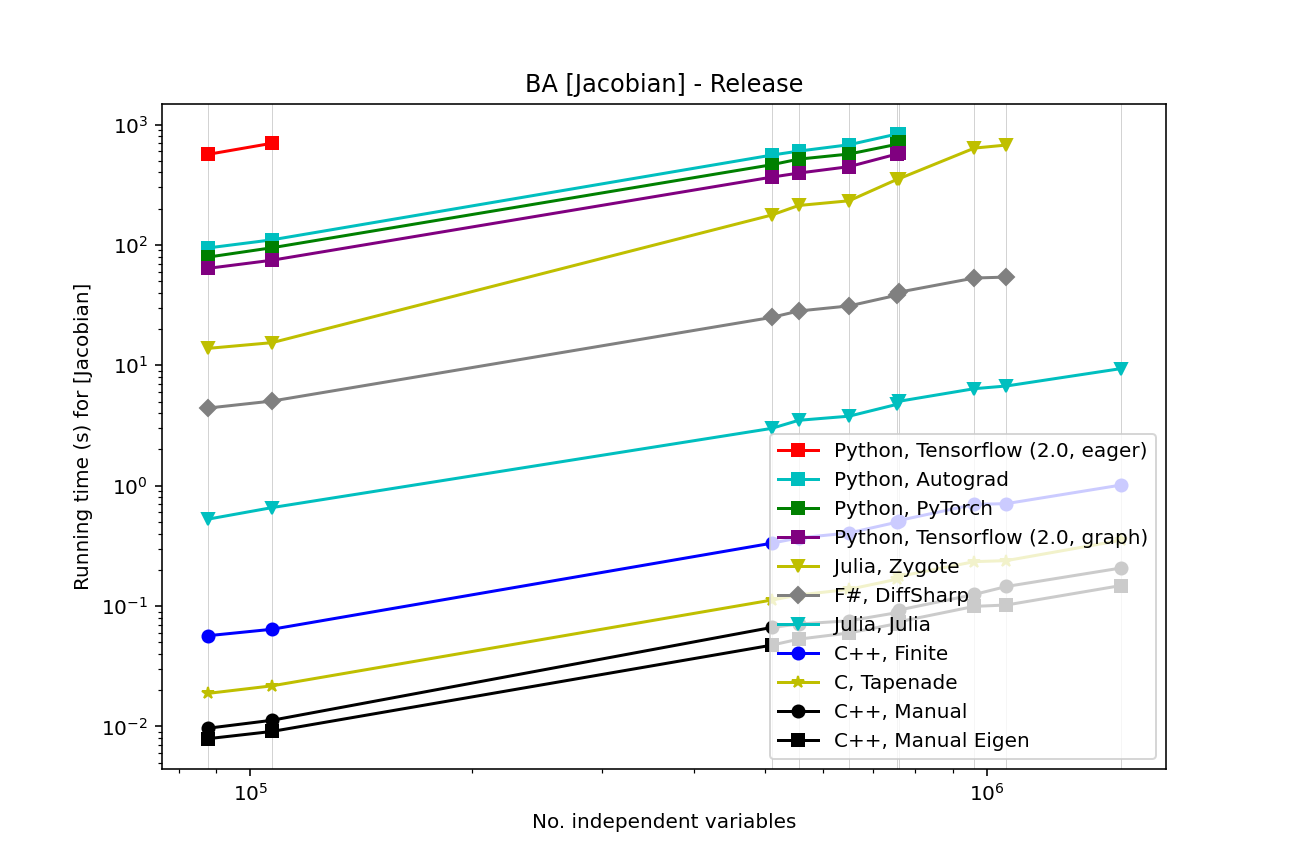
\includegraphics[width=0.5\columnwidth,trim={0 1cm 1cm 1.7cm},clip]{ba-jacobian-adbench.png}}
    \caption{The bundle adjustment benchmark (conducted by the ADBench project of microsoft).}\label{bench-ba}
\end{wrapfigure}
Tapenade is $10^{3-5}$ times faster than PyTorch and TensorFlow. However Tapenade is commercial, close sourced and C/Fortran based.
We are proud that NiLang is even better than Tapenade in this benchmark.
We strongly recommend referees to read the ADBench paper [arXiv:1807.10129], you will find that we have chosen one of the worlds' best generic AD package as our baseline.
We don't benchmark the popular Julia package Flux because we benchmarked its backend Zygote instead, where NiLang shows more than one order advantage in time.

Some referees are wondering if reversible computing is equivalent to traditional AD with optimized checkpointing.
We want to emphasis that reversible programming shows advantages in speed and memory mainly for one simple reason: \textit{the coding style and reversible thinking matters.}
In NiLang, it is hard to write ``bad'' code because every allocation must be explicit.
In the sparse matrix dot product example in the Appendix.
One has to preallocate a \texttt{branch\_keeper} to store the decisions of branches to enforce reversibility inside the loop.
If a user is writing it in freestyle, it impossible to avoid stack operations inside the loop and slow down the program.
Allocating automatically for a user is even more dangerous in GPU programming.
In NiLang, one can compile the bundle adjustment code to GPU to enjoy a ~200x speed up with no more than 10 extra lines of code.
It is easy to completely avoid allocation inside a loop in NiLang, but not for the optimal checkpointing, where a user does not have full control of the allocation and the reversibility is not fully exploited. Not to say optimal checkpointing itself is a well known hard topic.
Allocation can be the performance killer when one want to differentiate mutating array operations that many frameworks forbid such operations.
Some people use NiLang to differentiate backtest policies and variational mean field computing and increase the performance by a factor of $\sim600$ comparing with Zygote, because the mutating array is properly handled.
As far as we know, computational graph is not convenient to represent inplace operations.
Either the write-once \texttt{TensorArray} in TensorFlow or the mutable leaf tensors in PyTorch are not truly mutable.
This explains one of the referees' concern that the computational graph can represent any program.
Yes, but they are not convenient to describe mutating arrays.

%One of the referee mention that to handle the backward rule of ``+'' operation, one do not need to store the inputs of an instruction, gradient of both inputs are $1$. There is no need to trace back the state. We haven't put effort in optimizing such operations yet.
%In NiLang, the backward propagation program generally contains $\sim2$ times more instructions than the forward pass. This factor is estimated by considering the backward rule of the multiplication operation. This is a known bottleneck in the field of generic AD.

Some referees want to know from which aspect NiLang is different from a traditional reversible programming language.
For a long time, the reversible programming languages concern too much about theoretical elegance and ignored productivity. Researchers tried to add functional and object-oriented features to reversible languages.
NiLang is special for that it supports many practical elements like arrays, complex numbers, fixed-point numbers, and logarithmic numbers and being an eDSL so that it can be used directly to accelerate the Zygote framework in Julia.
And one of the referees is interested to know the limitations of NiLang. Reversible programming does not have any limitation in representing a computational process, because any program can be written reversibly. The most severe weakness of NiLang should be the floating-point arithmetic suffers from the rounding error.
We can ease this problem by combining fixed-point numbers and logarithmic numbers, which will be explained in the next update.

2/4 referees think our result can not be reproduced. Considering both NiLang and the benchmarks are open source on GitHub, we don't think this comment is justified.
We will address other comments like SVD is available in PyTorch and TensorFlow,
comparing reversible programming and the reversible neural networks in the main text directly. Thanks for your valuable information.

At last, we encourage referees to view this project more from the ``future'' perspective.
Nowadays, energy is becoming one of the most deadly bottlenecks for machine learning applications.
From a physicist's perspective, we believe that reversible computing is the only correct approach to solve energy conundrums.
Classical reversible computing has been silenced for $\sim$15 years, NiLang is trying to bridge the new trend machine learning and reversible computing.
We will try our best to convey this point better in the updated version. As one of the referees said, it is a long overdue.


\end{document}
